\chapter{Lec 11 - Generalized Linear Models and SVM II}
\section{SVM for non-separable case}
Let's extend the SVM model for non-separable data. With this approach we try to find a balance between maximizing the margin of the hyperplane and minimizing the number of misclassifications.\newline\newline
In the \textit{standard} SVM model, the solution is subject to the constraint that each point in the training set must be on the \textit{correct} side of the hyperplane:
\[\forall i \in \{1,...,n\}: y_{i}(\textbf{w} \cdot \textbf{x}_{i} + b) \geq 1\]
If the examples are not linearly separable we have to allow that some constraints are violated. This can be done by introducing \textit{slack} variables $\xi_{i} \geq 0$, $i = 1,...,n$, one for each constraint:
\[y_{i}(\textbf{w} \cdot \textbf{x}_{i} + b) \geq 1 - \xi_{i}\]
Basically, we replace the hard constraint with a softer one. These slack variables measure the distance between the point and the margin hyperplane where that point was supposed to be.
\begin{center}
    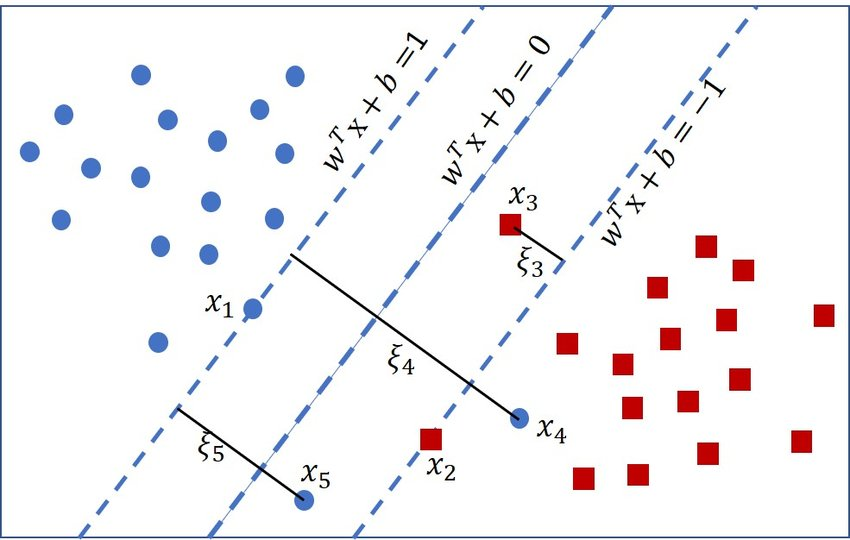
\includegraphics[scale = 0.7]{images/slack var.png}
\end{center}
We need to modify the cost function so to penalize slack variables which are not 0. Then, the \textbf{minimization} problem becomes the following:
\[\frac{1}{2}||\textbf{w}||^{2} + C\sum_{i = 1}^{n}\xi_{i}\]
where $C$ (regularization hyper-parameter) is a positive constant controlling the trade-off between the complexity of the hypothesis space and the number of margin errors.\newline\newline
The dual formulation is very similar to the one defined for separable data:
\[max_{\alpha} \sum_{i=1}^{n}\alpha_{i} - \frac{1}{2}\sum_{i,j=1}^{n}y_{i}y_{j}\alpha_{i}\alpha_{j}(\textbf{x}_{i}\cdot \textbf{x}_{j})\]
\[subject \,\, to: \,\, \forall i \in \{2,...,n\}: 0 \leq \alpha_{i} \leq C,\,\, and \quad \sum_{i=1}^{n}y_{i}\alpha_{i} = 0\]
The main difference between the two is due to the fact that the dual variables are upper bounded by $C$. The value of $b$ is obtained similarly to the separable case.\newline\newline
Note that a smaller C value results in a larger margin but allows for more misclassifications, while a larger C value results in a smaller margin but fewer misclassifications. This parameter can be seen as a way to control over-fitting, because increasing $C$ means to minimize the training error.\newline\newline
Nevertheless, this formulation is not always satisfactory because of the limited separation capability of a hyperplane (we are not able to perform non-liner separation of training data).
\section{Non-separable case: Another approach}
When the examples are not linearly separable the idea is to use a non-linear transformation in order to project all the points into a higher dimensional space.
\[\textbf{x} \rightarrow \phi(\textbf{x})\]
This approach is based on the following two steps:
\begin{enumerate}
    \item The input vectors (\textbf{input space}) are projected into a larger space (\textbf{feature space}). This is justified by Cover's theorem on separability, which states that non-linearly separable patterns may be transformed into a new feature space where the patterns are linearly separable with high probability, if the transformation is non-linear and if the dimensionality of the feature space is high enough.

    \item The optimal hyperplane in the feature space is computed.
\end{enumerate}
The hyperplane in the transformed space will correspond to a non-linear decision surface in the original space.\newline\newline
We can assume that any of the new feature space coordinate is generated by a non-linear function $\phi_{i}(\cdot)$. Given $M$ functions $\phi_{j}(\textbf{x})$ with $j = 1,...,M$, a generic vector $\textbf{x}$ is mapped into the following $M$-dimensional vector:
\[\phi(\textbf{x}) = [\phi_{1}(\textbf{x}),...,\phi_{M}(\textbf{x})]\]
A hyperplane in the feature space is defined as:
\[\sum_{j=1}^{M}w_{j}\phi_{j}(\textbf{x}) + b = 0\]
\[= \sum_{j = 0}^{M}w_{j}\phi_{j}(\textbf{x}) = \textbf{w} \cdot \phi(\textbf{x}) = 0\]
where $\phi_{0}(\textbf{x}) = 1$ and $w_{0} = b$\newline\newline
By changing the definition of the dual formulation, it follows that:
\[\textbf{w} = \sum_{k = 1}^{n}y_{k}\alpha_{k}\phi(\textbf{x}_{k})\]
The weight vector $\textbf{w}$ can be expressed as a linear combination of the $n$ training examples. So, the equation defining the hyperplane becomes:
\[\sum_{k = 1}^{n}y_{k}\alpha_{k}\phi(\textbf{x}_{k}) \cdot \phi(\textbf{x}) + b = 0\]
where $\phi(\textbf{x}_{k}) \cdot \phi(\textbf{x})$ represents the dot product \textbf{in feature space} between vectors induced by the $k$-th training instance and the input $\textbf{x}$.
\section{Kernel functions}
A Kernel function $K$ is a non-linear function whose result is equal to the dot-product in the feature space between two given vectors:
\[K(\textbf{x}_{k}, \textbf{x}) = \phi(\textbf{x}_{k}) \cdot \phi(\textbf{x}) = \sum_{j = 0}^{M} \phi_{j}(\textbf{x}_{k})\phi_{j}(\textbf{x}) = K(\textbf{x}, \textbf{x}_{k})\]
\textbf{Definition:}\newline
A kernel function is a function $K(\cdot, \cdot)$ such that for all $\textbf{x}, \textbf{z} \in X$, satisfies $K(\textbf{x}, \textbf{z}) = \phi(\textbf{x}) \cdot \phi(\textbf{z})$ where $\phi(\textbf{x})$ is a mapping from $X$ to a higher dimensional feature space $H$.\newline\newline
In general, a kernel function represents a dot-product between vectors generated by some non-linear transformation.\newline\newline
Function with this property do actually exists, if some conditions are satisfied (Mercer's conditions). Note that it's not guaranteed that for all non-linear transformations $\phi$ it exists such a function $K$.\newline\newline
Examples of popular kernel functions:
\begin{itemize}
    \item linear kernel, $K(\textbf{x},\textbf{z}) = x \cdot z$
    \item polynomial kernel of degree $p$, $K(\textbf{x},\textbf{z}) = (\textbf{x} \cdot \textbf{z} + u)^{p}$, $u > 0$
    \item Exponential kernel, $K(\textbf{x},\textbf{z}) = exp(\textbf{x} \cdot \textbf{z})$
    \item Radial-basis function (RBF) kernel, $K(\textbf{x},\textbf{z}) = exp(-\gamma ||\textbf{x} - \textbf{z}||^{2}),\,\, \gamma > 0$
\end{itemize}
if we get such a (symmetric) function, we could compute the decision function on feature space \textbf{without} explicitly representing the vectors into the feature space (we do not need to know anything about the non-linear transformation $\phi$).
\section{SVM problem formulation with Kernel}
The introduction of a kernel, actually, does not modify the problem formulation:
\[max_{\alpha}\sum_{i=1}^{n}\alpha_{i} - \frac{1}{2}\sum_{i,j}^{n}y_{i}y_{j}\alpha_{i}\alpha_{j}K(\textbf{x}_{i}, \textbf{x}_{j})\]
\[subject \,\, to: \,\, \forall i \in \{1,...,n\} : 0 \leq \alpha_{i} \leq C \,\, and \,\, \sum_{i=1}^{n}y_{i}\alpha_{i} = 0\]
Basically, all the occurrences of the dot-product between transformed examples are replaced with the kernel function. The needed kernel values are computed over all pairs of vectors $K(\textbf{x}_{i}, \textbf{x}_{j})$, with $i,j = 1,...,n$ and arranged into a matrix $\textbf{K} \in \mathbb{R}^{n \times n}$ (where $n$ is the number of examples) known as \textbf{kernel matrix} or \textbf{gram matrix}.\newline\newline
\textbf{Definition:}\newline
The Gram (or kernel) matrix associated with the kernel function $K(\cdot, \cdot)$, evaluated on a finite subset of examples $X = \{\textbf{x}_{1},...,\textbf{x}_{n} \in X\}$, is the matrix $\textbf{K} \in \mathbb{R}^{n \times n}$ such that:
\[\textbf{K}_{i,j} = K(\textbf{x}_{i}, \textbf{x}_{j})\]
For example, if we use a polynomial kernel with degree $p = 3$ we obtain that $\textbf{K}_{i,j} = (\textbf{x}_{i} \cdot \textbf{x}_{j} + 1)^{3}$. Therefore, a new instance $\textbf{x}$ is classified by the following discriminant function:
\[h(\textbf{x}) = sign( \sum_{\textbf{x}_{k} \in SV}y_{k}\alpha_{k}^{*}K(\textbf{x}_{k}, \textbf{x})) = sign(\sum_{\textbf{x}_{k} \in SV}y_{k}\alpha_{k}^{*}(\textbf{x}_{k} \cdot \textbf{x} + 1)^{3})\]
With this approach, we can use a non-linear transformation $\phi(\cdot)$ \textbf{implicitly}, in fact, what we need is not the explicit representation of vectors in feature space, but their dot-product into the feature space. This can be directly computed in the input space using the kernel function.\newline\newline
Note that the formulation with kernel works only with respect to the dual formulation of the SVM problem. This is because in the primal formulation the decision function does not depend only on dot-products between examples, but we have to minimize a vector of weights $\textbf{w}$.

\section{Polynomial kernel}
Given two vectors $\textbf{x}$ and $\textbf{z}$ and the following mapping $\phi()$
\[\textbf{x} = (x_{1}, x_{2}); \,\, \phi(\textbf{x}) = (x_{1}^{2}, x_{2}^{2}, \sqrt{2}x_{1}x_{2})\]
\[\textbf{z} = (z_{1}, z_{2}); \,\, \phi(\textbf{z}) = (z_{1}^{2}, z_{2}^{2}, \sqrt{2}z_{1}z_{2})\]
A dot product between $\phi(\textbf{x})$ and $\phi(\textbf{z})$ corresponds to evaluate the function $K_{2}(\textbf{x},\textbf{z}) = \langle x, z\rangle^{2}$, which is the polynomial kernel of degree 2:
\[\langle \phi(\textbf{x}), \phi(\textbf{z}) \rangle\ = \langle (x_{1}^{2}, x_{2}^{2}, \sqrt{2}x_{1}x_{2}), (z_{1}^{2}, z_{2}^{2}, \sqrt{2z_{1}z_{2}})\rangle\]
\[= x_{1}^{2}z_{1}^{2} + x_{2}^{2}z_{2}^{2} + 2x_{1}z_{1}x_{2}z_{2}\]
\[= \langle x, z \rangle^{2}\]
\[= (x_{1}z_{1} + x_{2}z_{2})^{2}\]
\[= K_{2}(\textbf{x},\textbf{z})\]
$K_{2}()$ is faster to evaluate than the dot-product between transformed vectors $\langle \phi(\textbf{x}), \phi(\textbf{z}) \rangle $\newline\newline
This demonstration shows that we can see the polynomial kernel as a dot-product in this specific feature space between two vectors.

\section{Representation with kernels}
A kernel function $K: X \times X \rightarrow \mathbb{R}$ can be seen as a (symmetric) function that gives, for a given pair of examples, a real value which represents the similarity between them. For example, let's consider the Radial-basis kernel:
\[K(\textbf{x}_{i},\textbf{x}_{j}) = exp(-\gamma ||\textbf{x}_{i} - \textbf{x}_{j}||^{2}),\,\, \gamma > 0\]
Note that when $\textbf{x}_{i} = \textbf{x}_{j}$ $K(\textbf{x}_{i},\textbf{x}_{j})$ is closed to 1, and when $\textbf{x}_{i} \neq \textbf{x}_{j}$ it tends to 0. So, given an object $S = \{x_{1}, x_{2},...,x_{n}\}$, it can be represented by a symmetric matrix $\textbf{K} = [K(x_{i}, x_{j})]_{i,j} \in \mathbb{R}^{n \times n}$. Basically, we build the kernel matrix $\textbf{K}$ by computing the kernel function on each possible pair of examples.\newline\newline
The \textbf{advantages} of using kernel matrices representation are different:
\begin{itemize}
    \item It allows you to build a pipeline in which you first compute the kernel matrix, with respect to your data, and then you change the learning algorithm (that takes as input this matrix) according to your needs. Basically, it improves the \textbf{modularity} of the system.

    \item The dimensionality of data depends on the number of objects and not on their vector dimensionality. This is because the kernel matrix is computed considering all the possible pairs of examples.

    \item Comparison between objects can result computationally simpler than using the explicit object representation.

    \item The implicit mapping of data into a higher-dimensional feature space can capture complex patterns and non-linear relationships in data.
\end{itemize}

\textbf{Disadvantages} of kernels are:
\begin{itemize}
    \item The memory space required to store the kernel matrix. In fact, the dimension of the matrix is squared with respect to the dimension of the training set.

    \item The time required to evaluate the scoring function is not suitable for real-time applications. This is because the scoring function is computed by evaluating many kernels.
\end{itemize}
Recently, there have been effort to \textit{linearize} the kernel. This can be done by approximating the kernel using a fine subset of non-linear features:
\[\langle \overline{\phi}(\textbf{x}), \overline{\phi}(\textbf{z}) \rangle\ \approx \langle \phi(\textbf{x}), \phi(\textbf{z}) \rangle = K(\textbf{x},\textbf{z})\]

\subsection{The Kernel Trick}
Any algorithm for vectorial data that can be expressed in terms of dot-products, can be implicitly executed in the feature space associated to a kernel by replacing dot-products with kernel evaluations. Two algorithms that can be \textbf{kernelized} are the Perceptron algorithm and k-NN.\newline\newline 
Moreover, by defining an appropriate kernel, we can apply algorithm for vectorial data (SVM, Perceptron, etc..) to non-vectorial data (strings, trees, sequances, etc..).\newline\newline
For example, in k-NN we need to compute the distances between examples, but if we want to compute the distances in the feature space we can use the kernel trick: Given two objects $x, z \in X$, the squared distance between the two objects in the feature space is computed by:
\[d(x,z)^{2} = ||\phi(x) - \phi(z)||^{2}\]
Computing the squared distance between two points corresponds to compute the squared norm of $\phi(x) - \phi(z)$.
\[= \phi(x) \cdot \phi(x) + \phi(z) \cdot \phi(z) - 2\phi(x) \cdot \phi(z)\]
\[= K(x, x) + K(z, z) - 2K(x, z)\]
That is:
\[d(x, z) = \sqrt{K(x, x) + K(z, z) - 2K(x, z)}\]
Note that the values of $\phi(x), \phi(z)$ are not explicitly used.

\section{Kernel properties and extensions}
Let $K_{1}, K_{2}$ be kernels defined on $X \times X$, $a \in \mathbb{R}^{+}$, $\phi : X \rightarrow \mathbb{R}^{N}$ with $K_{3}$ a kernel over $\mathbb{R}^{N} \times \mathbb{R}^{N}$:
\begin{itemize}
    \item $K_{1}(\textbf{x}, \textbf{z}) + K_{2}(\textbf{x}, \textbf{z})$ is a kernel.
    
    \item $aK_{1}(\textbf{x}, \textbf{z})$ is a kernel

    \item $K_{1}(\textbf{x}, \textbf{z}) \cdot K_{2}(\textbf{x}, \textbf{z})$ is a kernel

    \item $K_{1}(\phi(\textbf{x}), \phi(\textbf{z}))$ is a kernel
\end{itemize}
A kernel can be easily normalized such to have the norm of the transformed vector equals to one ($||\phi(\textbf{x}) = 1||$):
\[\tilde{K} = \frac{K(\textbf{x}, \textbf{z})}{\sqrt{K(\textbf{x},\textbf{x}) K(\textbf{z},\textbf{z})}}\]
Kernel definition can be extended to other types of inputs:
\begin{itemize}
    \item Kernel for strings
    \item Kernel for trees
    \item Kernel for graphs
\end{itemize}
